
\section{Modelo 2D simplificado}

Esta siguiente sección detallará el tratamiento matemático efectuado para controlar un vehículo con propulsión vectorizada en el plano. El proposito es ilustrar a un nivel simple las herramientas que serán aplicadas para controlar el vehículo diseñado.

\begin{figure}[htb!]
	\centering
	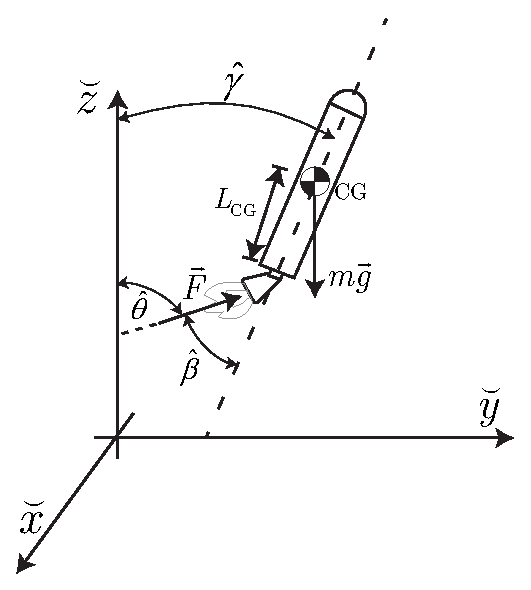
\includegraphics[width=9cm]{fig/rocketFBD.eps}
	\caption{Diagrama de cuerpo libre de un vehículo con propulsión vectorizada 2D.}
	\label{fig:FBD2D}
\end{figure}


\subsection{Modelado matemático}
Comenzamos con las ecuaciones dinámicas de un vehículo en el plano con control de propulsión vectorizada (por ángulo)

\[
\left\{
\begin{array}{l}
	\ddot{y}=\frac{F}{m} \sin(\gamma+\beta) \\
	\ddot{z}=\frac{F}{m} \cos (\gamma+\beta)-g \\
	\ddot{\gamma} = \frac{L_{\CG}\cdot F}{I_{xx}}\sin\beta
\end{array}
\right.
\]
donde \(\LCG\) y \(F\) están en función del tiempo, $m =m_0 - \int \dot{m} $ y $\theta = \gamma+\beta$. 

Vale la pena aclarar que no se tomarán en cuenta los siguientes efectos:
\begin{itemize}
	\item Fuerza de drag
	\item Viento
	\item \textit{Fuel sloshing}
	\item Efectos relativisticos
\end{itemize}

\subsection{Armado de sistema lineal}

Se propone un punto de operación alrededor del cual se linealizan las ecuaciones. El estado del vehículo es \textit{vertical y quieto en el espacio}. \footnote{La linealización esd valida solo para un vehículo vertical. Se debrá modificar el método para modelar un vehículo orbital.} 

\begin{align*}
	\gamma^* = 0 \\
	\beta^* = 0 \\
	F^* = mg
\end{align*}
en este caso $F$ es la desviación del punto de operación. Desde ahora en adelante $\Delta F = F- mg$.

\subsection{Representación en espacio de estados}
El número de variables de estado será igual a número de almacenadores de energía independientes. Estos son

\begin{enumerate}
	\item[$z$] Energía potencial por la gravedad
	\item[$\dot{y},\dot{z}$] Energía cinetica del vehículo
	\item[$\dot{\gamma}$] Momento angular del vehículo
\end{enumerate}
entonces, las variables de estado son las siguientes
\begin{align*}
	x_1 = y \\
	x_2 = \dot{y} \\
	x_3 = z \\
	x_4 = \dot{z} \\
	x_5 = \gamma \\
	x_6 = \dot{\gamma}
\end{align*}
donde $\dot{x_1} = x_2$, $\dot{x_3} = x_4$ y $\dot{x_5} = x_6$

Se aprovecha la expansión de Taylor para la linealización de expresiones trigonométricas:
\[
\sin(x+y)|_{x=x_0+\Delta x,y=y_0+\Delta y} \approx \sin(x_0+y_0) + \cos(x_0 + y_0) (x-x_0) + \cos(x_0 + y_0) (y-y_0)
\]

Las ecuaciones dinámicas de los estados 2,3, y 4 son dadas por las ecuaciones mostradas al comienzo de esta sección.
Abajo están las ecuaciones de estados
\begin{equation}
	\dot{x_2} = \frac{F}{m} \left( \gamma+\beta \right) = g x_5 + g u_2 
\end{equation}
\begin{equation}
\dot{x_4} = \frac{F}{m} - g =\frac{F-F_0}{m}= \frac{u_1}{m}
\end{equation}
\begin{equation}
\dot{x_6} = \frac{\LCG \cdot F}{I_{xx}} \beta = \frac{\LCG \cdot mg}{I_{xx}} u_2 
\end{equation}

donde $\Ts$ es el periodo de sampleo.

Los vectores de entrada y salida son
\[
\Cme{u}(t) = \begin{bmatrix}
u_1 \\
u_2
\end{bmatrix} = \begin{bmatrix}
\Delta F \\
\beta
\end{bmatrix}
\]
\[
\Cme{y}(t) = \begin{bmatrix}
y_1 \\
y_2 \\
y_3
\end{bmatrix} = \begin{bmatrix}
y \\
z \\
\gamma
\end{bmatrix}
\]
tal que las ecuaciones de salida son

\begin{equation}
	y_1 = x_1 
\end{equation}
\begin{equation}
	y_2 = x_3
\end{equation}
\begin{equation}
	y_3 = x_5
\end{equation}

Se escriben las matrices del sistema y de control ($\Mme{D} = [0]$)
\begin{equation} \label{eq:ssmatrices}
	\Mme{A} = 
	\left[\begin{array}{cccccc} 0 & 1 & 0 & 0 & 0 & 0\\ 0 & 0 & 0 & 0 & g & 0\\ 0 & 0 & 0 & 1 & 0 & 0\\ 0 & 0 & 0 & 0 & 0 & 0\\ 0 & 0 & 0 & 0 & 0 & 1\\ 0 & 0 & 0 & 0 & 0 & 0 \end{array}\right],\quad \Mme{B} = 
	\left[\begin{array}{cc} 0 & 0\\ 0 & g\\ 0 & 0\\ \frac{1}{m} & 0\\ 0 & 0\\ 0 & \frac{\LCG \cdot mg}{I_{xx}} \end{array}\right], \quad \Mme{C} =  \left[\begin{array}{cccccc} 1 & 0 & 0 & 0 & 0 & 0\\ 0 & 0 & 1 & 0 & 0 & 0\\ 0 & 0 & 0 & 0 & 1 & 0 \end{array}\right]
\end{equation}
El sistema mostrado en \eqref{eq:ssmatrices} es \textit{fully state controllable}.